%%%%%%%%%%%%%%%%%%%%%%%%%%%%%%%%%%%%%%%%%%%%%%%%%%%%%%%%%%%%%%%%%%%%%%%%%%%%%
%	e-Yantra, IIT-Bombay

%	Document Author: Chinmay Patil
%	Date: 11-July,2016
%	Last Edited by: Chinmay
%   Date Last updated: 11-06-2016 

%%%%%%%%%%%%%%%%%%%%%%%%%%%%%%%%%%%%%%%%%%%%%%%%%%%%%%%%%%%%%%%%%%%%%%%%%%%%%


\documentclass[11pt,a4paper]{article}
\usepackage{graphicx}
\usepackage{listings}
\usepackage{graphics}
\usepackage{wrapfig}
\usepackage[T1]{fontenc}
\usepackage[margin=1.2in]{geometry}
\usepackage{tcolorbox}
\usepackage{hyperref}
\usepackage{dingbat}
\usepackage{float}
\usepackage{tocloft}

\begin{document}
\begin{titlepage}
\title{Installation Procedure and first run of Wiced Sense on Ubuntu}
\author{e-Yantra Team}
\date{\today}
\maketitle
\end{titlepage}

    %\renewcommand\cftloftitlefont{\LARGE}
    \tableofcontents
    \newpage
	\section{Overview}
	 {\Large \hspace{7mm} Wiced sense is a Bluetooth Low Energy device. It incorporates five Microelectromechanical sensors namely,
	 \begin{itemize}
	 \\\item Gyroscope (L3GD20)\\ \item Accelerometer (LIS3DSH)\\\item eCompass (LSM303D)\\\item Pressure sensor (LPS25H)\\\item Humidity Temperature sensor (HTS221).
	 \end{itemize}\\ \\The data from these sensors is transmitted via bluetooth to any low energy compatible device i.e which has a bluetooth version 4 or above.
	 This tutorial will provide detailed procedure for installing all the packages required to acquire the data from the Wiced Sense tag by Broadcom on the local system (Ubuntu).}
	 
	\newpage
	\section{Prerequisites}
	\begin{itemize}
	\item Knowledge about installing Ubuntu on a system.
	\item Commands required for doing tasks in terminal.
	\item A good Internet Connection.
	\end{itemize}
	
	\section{Hardware Requirement}
	\begin{itemize}
	\item Wiced Sense Tag
	\item A local system (Laptop or PC with bluetooth 4.0 or above)
	\end{itemize}
	
	\section{Software Requirement}
	\begin{itemize}
	\item Ubuntu 16.04 running on local system.
	\end{itemize}
	
	\newpage
	\section{Installation Procedure}
	
	\begin{itemize}
	\begin{figure}[h]
    \centering
	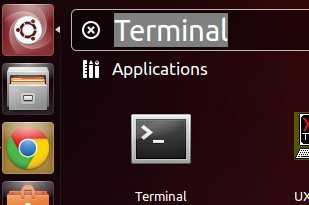
\includegraphics[scale=0.5]{terminal.jpg}
	\end{figure}
	\item Open the Dash by clicking the Ubuntu icon in the upper-left, type "terminal",and select the Terminal application from the results that appear.
	\item Open the terminal and update the system by typing 
	 "sudo apt-get update".
	 \item Upgrade the system by typing  "sudo apt-get upgrade"
	 \newpage
	 \begin{figure}[h]
    \centering
	
\includegraphics[scale=0.5]{nodejs.png}
	\end{figure}
	 \item What is node js ?
	 	\begin{itemize}
	 	\item Node.js is a platform built on Chrome's JavaScript runtime for easily building fast and scalable network applications. Node.js uses an event-driven, non-blocking I/O model that makes it lightweight and efficient, perfect for data-intensive real-time applications that run across distributed devices.
	 	\item An important thing to realize is that Node is not a webserver. By itself it doesn't do anything. It doesn't work like Apache. There is no config file where you point it to you HTML files. If you want it to be a HTTP server, you have to write an HTTP server (with the help of its built-in libraries). Node.js is just another way to execute code on your computer. It is simply a JavaScript runtime.
	 	\end{itemize}
	 
	 	\item Features of Node.js
	 	\begin{itemize}
	 	\item Asynchronous and Event Driven. All APIs of Node.js library are asynchronous that is, non-blocking. It essentially means a Node.js based server never waits for an API to return data. The server moves to the next API after calling it and a notification mechanism of Events of Node.js helps the server to get a response from the previous API call.

        \item Very Fast Being built on Google Chrome's V8 JavaScript Engine, Node.js library is very fast in code execution.

        \item Single Threaded but Highly Scalable - Node.js uses a single threaded model with event looping. Event mechanism helps the server to respond in a non-blocking way and makes the server highly scalable as opposed to traditional servers which create limited threads to handle requests. Node.js uses a single threaded program and the same program can provide service to a much larger number of requests than traditional servers like Apache HTTP Server.

        \item No Buffering - Node.js applications never buffer any data. These applications simply output the data in chunks.

        \item License - Node.js is released under the MIT license.
        	\end{itemize}
	 	
	 \item Install node js by typing "sudo apt-get install nodejs"

	 \item BlueZ is the official Linux Bluetooth protocol stack. It is an Open Source project distributed under GNU General Public License (GPL).
	 Development files for using the BlueZ Linux Bluetooth library can be installed by\\ "sudo apt-get install libbluetooth-dev"
	 \newpage
	 \begin{figure}[h]
    \centering
	
\includegraphics[scale=0.3]{npm-logo.png}
	\end{figure}
	
	\item NPM is Node Package Manager which provides following two main functionalities:
	\begin{itemize}
	\item  Online repositories for node.js packages/modules which are searchable on search.nodejs.org.
	\item  Command line utility to install Node.js packages, do version management and dependency management of Node.js packages.
	\item Install npm by typing "sudo apt-get install npm"
	\end{itemize}
	
	\item Next we need to create a symbolic link between node js and node. This can be done by : 
	"sudo ln -s /usr/bin/nodejs /usr/bin/node"
	\item Then we install userspace USB programming library development files by \\ "sudo apt-get install libusb-1.0-0-dev"
	\item Installing node-gyp 
	\begin{itemize}
	Node-gyp is a cross-platform command-line tool written in Node.js for compiling native addon modules for Node.js. It bundles the gyp project used by the Chromium team and takes away the pain of dealing with the various differences in build platforms. It is the replacement to the node-waf program which is removed for node v0.8.\\
	Node-gyp can be installed by typing "sudo npm install node-gyp -g"
	\end{itemize}
	\item Installing libudev-dev
	\begin{itemize}
     udev is a device manager for the Linux kernel. On Unix and Unix-like systems, hardware devices are accessed through special files (also called device files or nodes) located in the /dev directory. These files are read from and written to just like normal files, but instead of writing and reading data on a disk, they communicate directly with a kernel driver which then communicates with the hardware. 
     libudev provides APIs to introspect and enumerate devices on the local system.\\
     libudev-dev can be installed by typing "sudo apt-get install libudev-dev"
	\end{itemize}

	\newpage
	\item Installing Cylon js
		 \begin{figure}[h]
    \centering
	
\includegraphics[scale=0.3]{CylonJS.png}
	\end{figure}
    \begin{itemize}
\item 	Cylon.js is a JavaScript framework for robotics, physical computing, and the Internet of Things. It makes it incredibly easy to command robots and devices.
	We need Cylon NPM module to get started. 
	\item Cylon npm module can be installed by "sudo npm install cylon -g"
	\item Cylon.js has an extensible system for connecting to hardware devices. Compatiblity of the hardware can be found at https://cylonjs.com/
	\item Cylon js supports wiced sense. It has support to BLE (Bluetooth Low Energy) devices.
	\end{itemize}
	
	\item Installing Cylon BLE
	\begin{figure}[h]
    \centering
	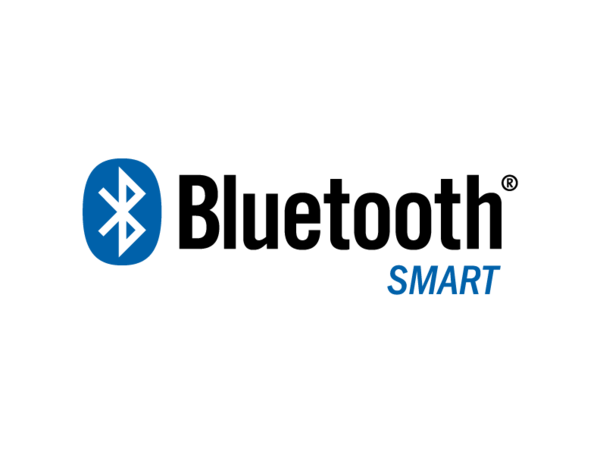
\includegraphics[scale=0.3]{bluetooth-smart.png}
	\end{figure}
	    \begin{itemize}  
	    \item Bluetooth Low Energy (BLE) is a newer standard for communicating with Bluetooth devices. It's focused on lower cost and power consumption. A number of newer hardware devices come with BLE on-board.

\item Cylon-ble module can be used to communicate directly with BLE devices, requesting low-level details such as battery status and generic device info. It can also be used as an adaptor for more complicated modules that control larger-scale devices, such as the Orbotix Ollie.
\item Cylon-ble module can be installed by command,\\
"sudo npm install cylon-ble -g"
\item We will now use cylon-ble modules's included commands to scan for BLE devices, and then to list the various BLE characteristics for a specific device.
\item A computer with a hardware adaptor that supports Bluetooth LE, also known as Bluetooth 4.0, or Bluetooth Smart is needed.
\end{itemize}
\newpage
\item Output after running cylon-ble-scan and cylon-ble-info. Ensure that u have pressed the 'Wake Button' and red led is glowing on wiced sense.
\begin{figure}[h]
    \centering
	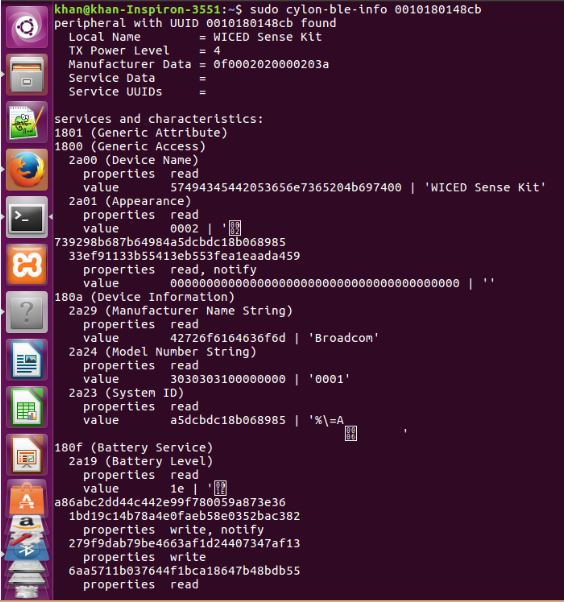
\includegraphics[scale=0.8]{info.JPG}
	\caption{ble-info}
	\end{figure}
\newpage
\item Understandng the code.
\begin{figure}[h]
    \centering
	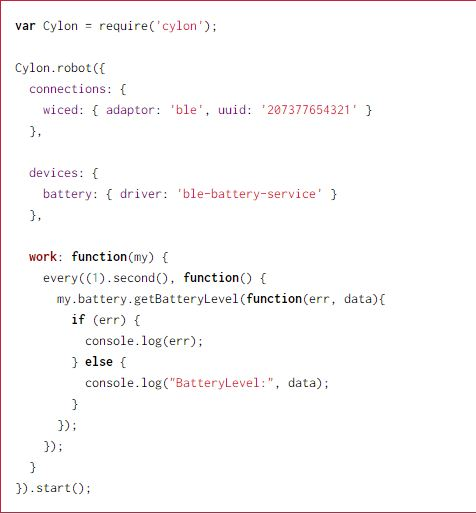
\includegraphics[scale=0.8]{ble.JPG}
	\end{figure}
     
     \item Node.js uses a module architecture to simplify the creation of complex applications. Modules are akin to libraries in C, or units in Pascal. Each module contains a set of functions related to the "subject" of the module. Cylon module is used here to communicate with the ble device.
     
     \item Adaptor used here is ble which we have just installed. The UUID ( universally unique identifier) is device specific and is different for every device.The intent of UUIDs is to enable distributed systems to uniquely identify information without significant central coordination.
     
     \item Note the UUID of the device that u got during the cylon-ble-scan. Copy that UUID and place it in this code.
     
     \item The driver 'ble-battery-service' is used to get the battery level of the device. Other drivers that can be used are "ble-characteristic",'ble-device-information' and 'ble-generic-access'.
     
     \item "console.log("BatteryLevel:", data);" prints the data on the console log. In this case it prints the battery voltage of the wiced sense.
     
     \item "every((1).second()," This invokes the function every 1 second.
	 \item Changes in the exsisting codes :
	  \begin{itemize}
	 \item Change the "adapter:central" to "adapter:ble"
	 \item Delete the "
	 \end{itemize}
	\newpage
	\item Installing cylon-wiced-sense
	 \begin{itemize}
	\item For installing cylon-wiced-sense adapter run the following command,\\
	"sudo npm install cylon-wiced-sense -g"
	\item Make sure that u have pressed the wake button on wiced sense.
	\item Pair the wiced sense by opening bluetooth settings.
	\item Now to acquire data from the wiced sense we need to run this code. Change the directory to ///////////// in which wiced-sense.js is located.
	Open terminal and type "sudo node wiced-sense.js".
	
	\item Output of the command is as follows.
	\end{itemize}
	\begin{figure}[h]
    \centering
	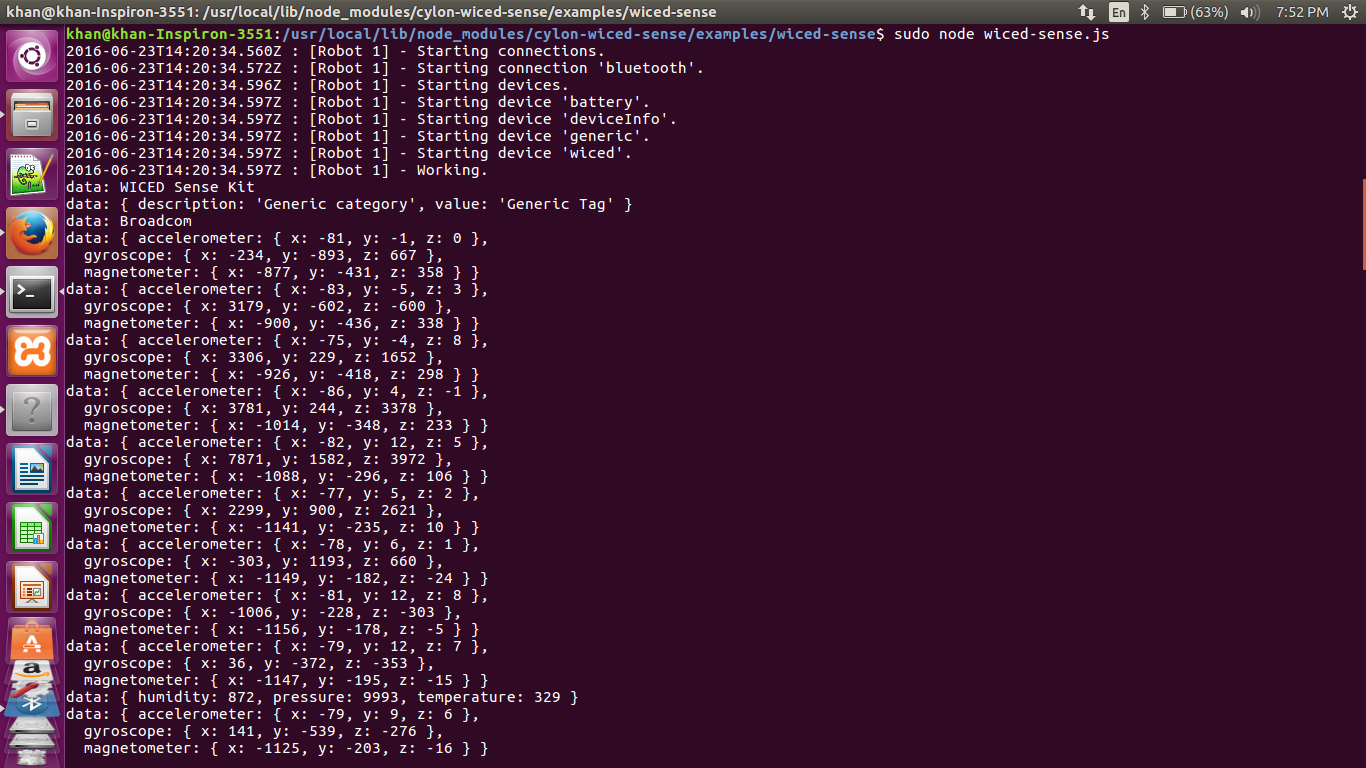
\includegraphics[scale=0.35]{ble-data.png}
	\end{figure}
    \end{itemize}
    
    
    \newpage
	\section{References}
	 \begin{itemize}
	 \item https://cylonjs.com/documentation/platforms/ble/
	     \item https://github.com/hybridgroup/cylon-ble
	         \item http://code.tutsplus.com/tutorials/nodejs-for-beginners--net-26314
	         \item http://www.signal11.us/oss/udev/
	     \end{itemize}

\end{document}



